%XeLaTeX
\documentclass{article}
\usepackage{lscape}

\setlength{\emergencystretch}{100pt}
\usepackage{tocloft}
\cftsetindents{subsubsection}{3em}{7em}
\cftsetindents{subsection}{3em}{6em}
\cftsetindents{section}{3em}{6em}
\usepackage[dvipsnames]{xcolor}
\usepackage{eso-pic,graphicx}
\usepackage[top=35mm, bottom=37mm, outer=27mm, inner=27mm, landscape]{geometry}
\setlength{\columnsep}{70pt}
\color{White}

\usepackage{fancyhdr}


\AddToShipoutPictureBG{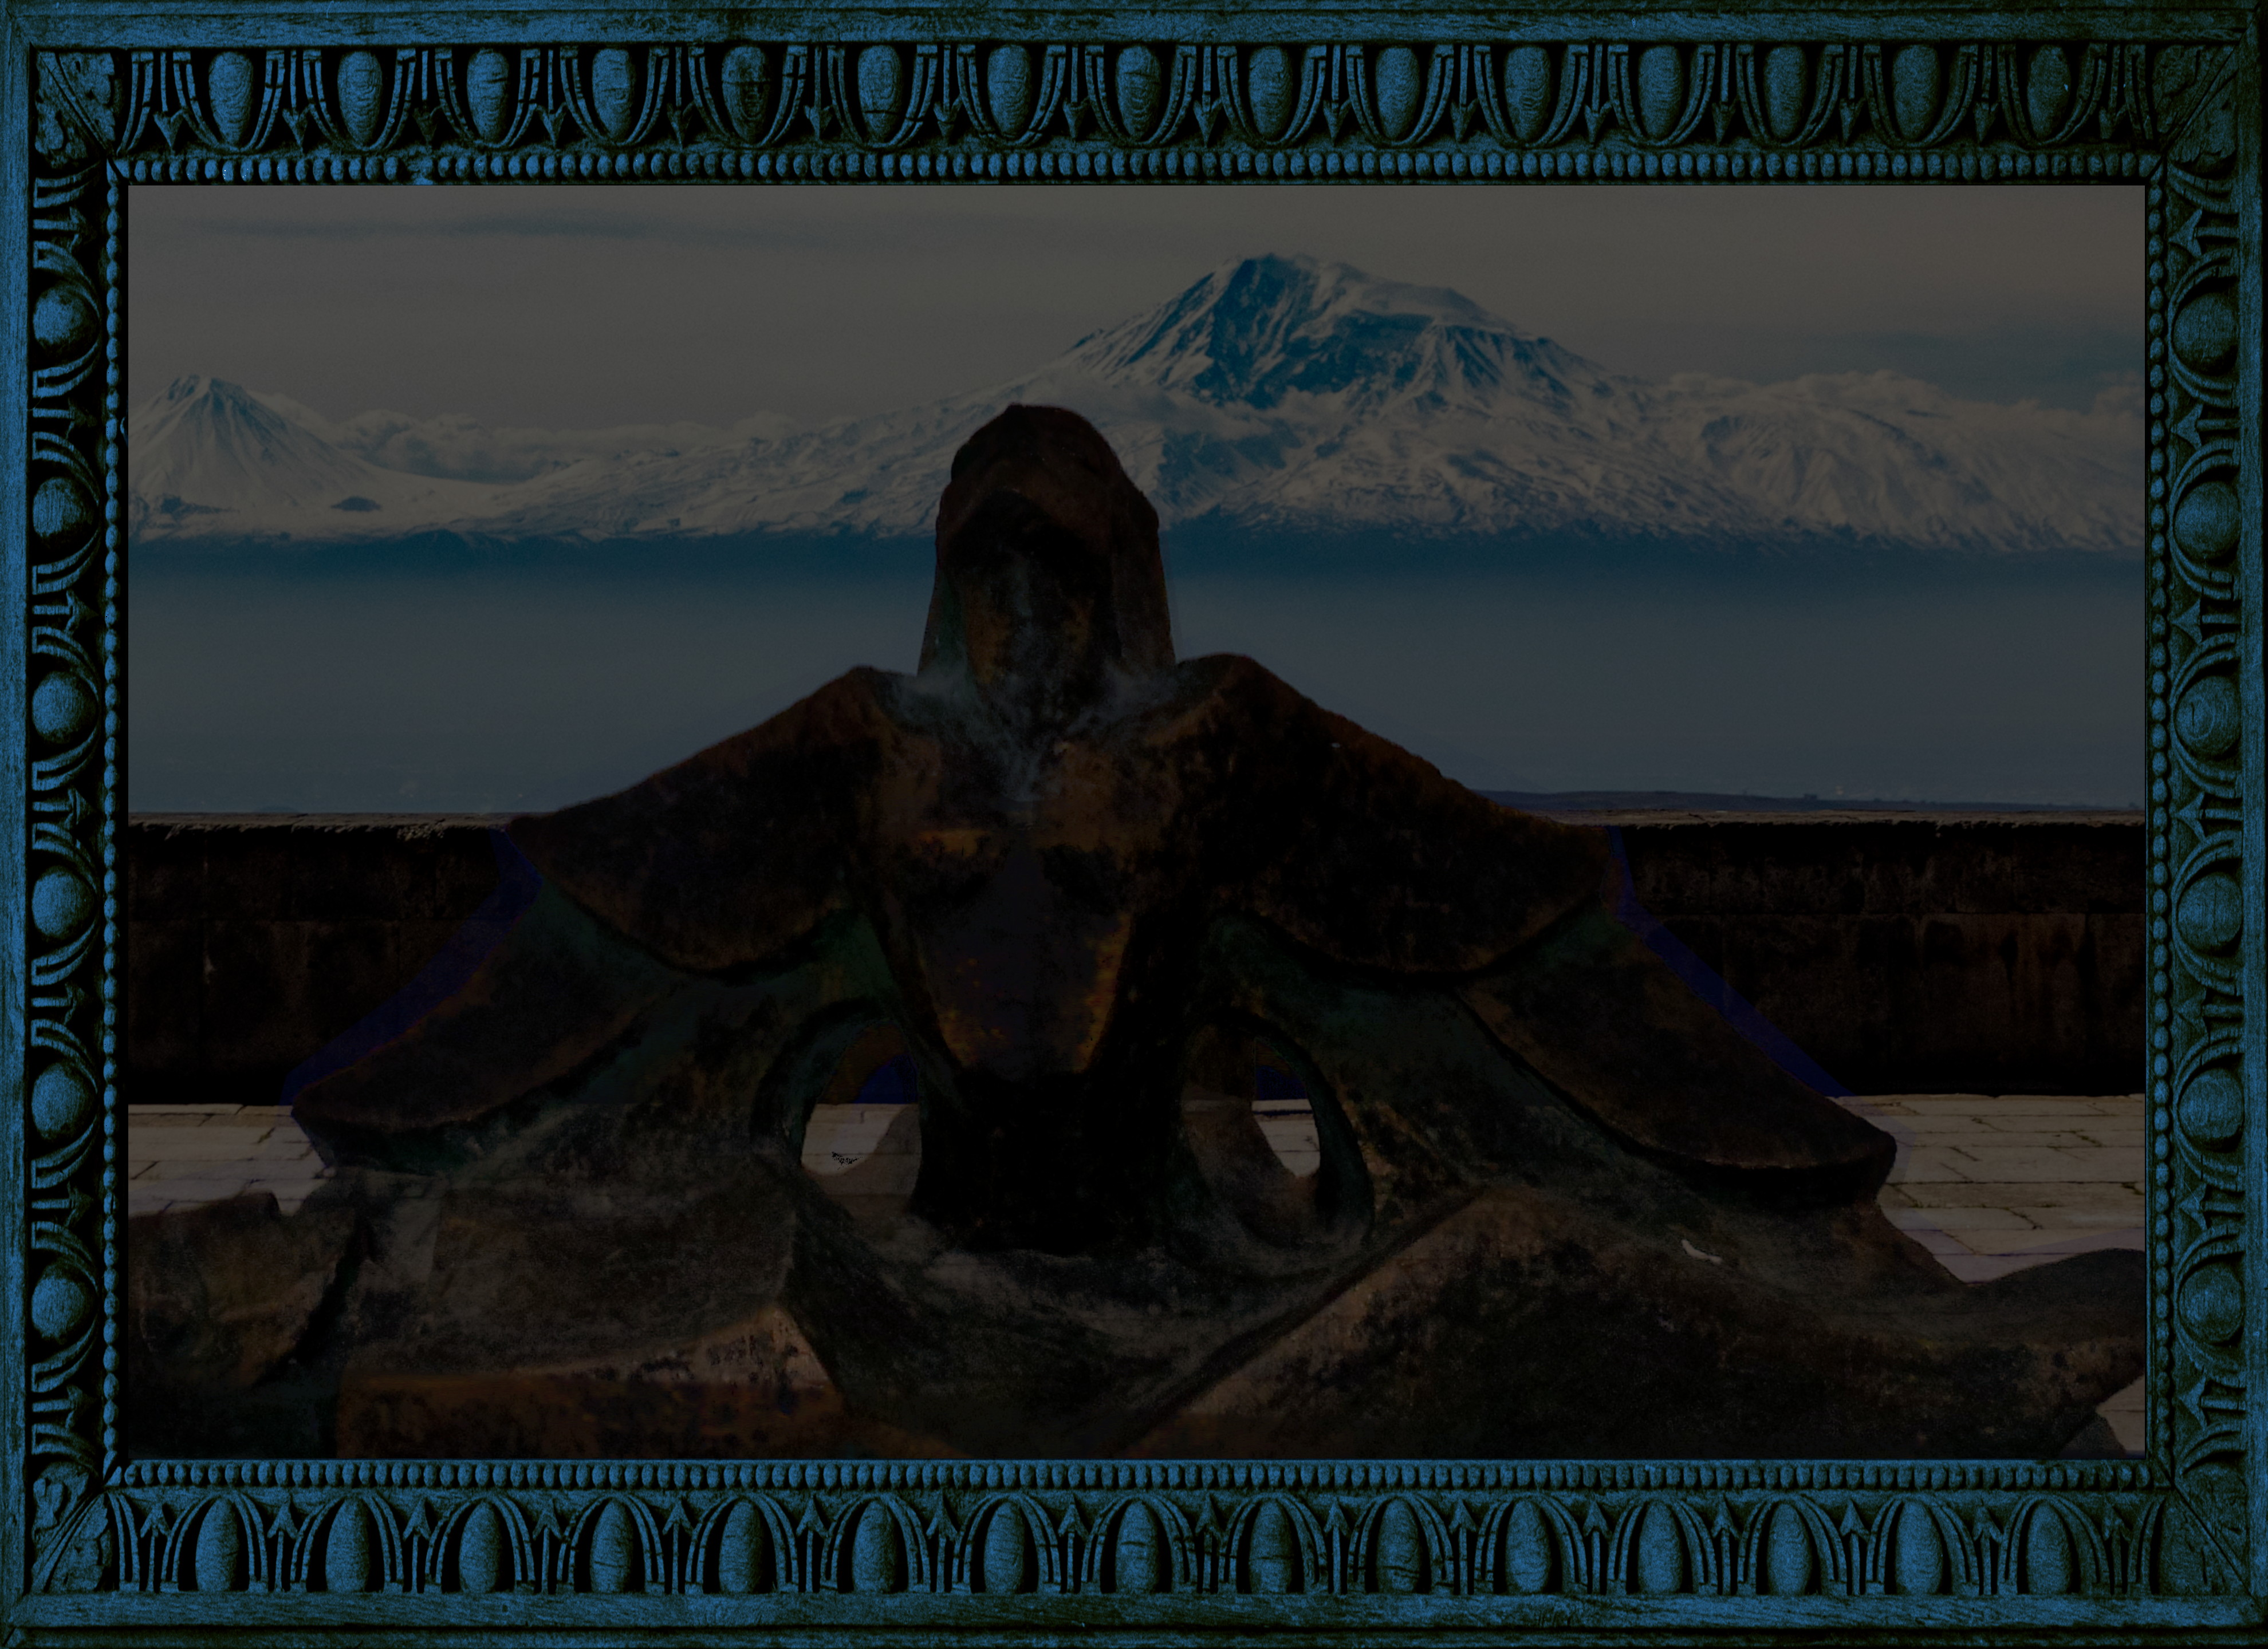
\includegraphics[width=\paperwidth,height=\paperheight]{ara2new.jpeg}}
\usepackage{microtype}

\usepackage{fontspec}
\usepackage{polyglossia}
\setdefaultlanguage{german}
\setotherlanguages{armenian,russian}

\setmainfont{Hianali}
\setsansfont{Hianali}
\setmonofont{Hianali}
%\newfontfamily{\arm}[Script=Armenian]{DejaVuSans}
%\newfontfamily{\arm}[Script=Armenian]{GHEA Grapalat}%monotonic greek only
%\newfontfamily{\armitalic}[Script=Armenian]{GHEA Grapalat}%monotonic greek only
\newfontfamily{\arm}[Script=Armenian]{Hianali}
\newfontfamily{\armitalic}[Script=Armenian]{Hianali}
\newfontfamily{\armenianfontsf}[Script=Armenian]{Hianali}
\newfontfamily\cyrillicfontsf{EB Garamond SC}
\newfontfamily\greekfontsf{EB Garamond SC}
%\newfontfamily{\arm}[Script=Armenian]{DejaVuSans-Bold}
%\newfontfamily{\armitalic}[Script=Armenian]{DejaVuSans-BoldOblique}
\defaultfontfeatures{Scale=MatchLowercase}
\pagestyle{fancy}
\fancyfoot[C]{\arm{\thepage}}
\fancyhead{}

\begin{document}

\renewcommand\thefootnote{{\small{\arabic{footnote}}}}
\let\oldfootnote\footnote
    \renewcommand{\footnote}[1]{\oldfootnote{{\normalsize#1}}}
\begin{titlepage} % Suppresses headers and footers on the title page
	\centering % Centre everything on the title page
	%\scshape % Use small caps for all text on the title page

	%————————————————
	%	Title
	%————————————————

	\rule{\textwidth}{1.6pt}\vspace*{-\baselineskip}\vspace*{2pt} % Thick horizontal rule
	\rule{\textwidth}{0.4pt} % Thin horizontal rule
	
	\vspace{1\baselineskip} % Whitespace above the title
	
	{\scshape\Huge \arm{Շամիրամի Առասպելը}}
	
	\vspace{1\baselineskip} % Whitespace above the title

	\rule{\textwidth}{0.4pt}\vspace*{-\baselineskip}\vspace{3.2pt} % Thin horizontal rule
	\rule{\textwidth}{1.6pt} % Thick horizontal rule
	
	\vspace{1\baselineskip} % Whitespace after the title block
	
	%————————————————
	%	Subtitle
	%————————————————
	

        {\large \arm{Գրեց Մանուկ Աբեղյան}}
 ‌
	%————————————————
	%	Editor(s)
	%————————————————
        \vspace*{\fill}    

        \vspace{1.0\baselineskip}

        { \arm{Արարատ: Ամսագիր կրօնական, պատմական, բանասիրական եւ բարոյական գիտելեաց}}
        
	\vspace{1\baselineskip}

        {\small\arm{Էջմիածին} 1901}
		
	\vspace{0.25\baselineskip} % Whitespace after the title block

        {\scshape\small \arm{Solar Anamnesis Edition}}% Publication year}
    
	{\scshape\footnotesize \arm{Attribution-ShareAlike 4.0 International}} % Publisher
\end{titlepage}
\clearpage
\twocolumn
\paragraph{}
\arm{\emph{Աղբիւրը}: — Շամիրամի և Արայ գեղեցկի մասին պատմելիս (Ա. ժե.) Խորենացին աղրիւր չէ յիշում, ոչ Մար Աբաս և ոչ առասպել կամ երգ:\footnote{Տես «ի բանսն՝ որ զնմանէ» խօսքի և «բանք» բառի բացատրութիւնը Բ. Գլ.} Բայց, ինչպէս արդէն տեսելենք (Ը. գլ.), ուրիշ աեղից գիտենք, որ «ի Հայկայ մինչև ցԱրայն Գեղեցիկ, զոր սպանեալ կաթոտն Շամիրամ» (Ա. ե.), ուստի և Արայի պատմութիւնն առնուած է Մար Աբասից: ԺԷ. գլխի մէջ ևս, ուր պատմուած է Շամիրամի կոտորելն իւր որդիներին, նորա կրիւը Ջրադաշտի հետ և փախուստը Հայաստան և նորա սպանուելն իւր որդի Նինուասից, աղբիւր չէ յիշուած: Բայց յաջորդ ԺԸ. գլխի մէջ յայտնում է, որ այդ պատմութիւնն առած է Մար Աբասից: Այդ գլխի վերնագիրն է. «Յաղագս թէ \emph{որպէս} հաւաստի նախ լեալ պատերազմ նորա ի Հնդիկս և զկնի \emph{մահուան} (մահ) նորա ի Հայս,»\footnote{N° 1671 Ա. ձեռագիր. միւս Ա. ձեռագիրները «որպես» բաոը չունին. իսկ N°N° 1665, 616 «մահուան» ձեւի փոխանակ ունին «մահ,» որ աւելի ուղիղ ե քերականօրեն: Շարունակութիւնն ևս աոնում ենք N° 1671 ձեռագրից, որին համեմատ են միւս Ա. ձեռագիրները չնչին տարբերութիւններով: Տպագիրն աղաւաղուած ե, չունենաշով Շամիրամի պատերազմը Ջրադաշտի հետ և սորան յաղթելը:} այսինքն թէ ինչպէս Շամիրամի պատերազմը Հնդկաստանում հաւաստաւ առաջ է եղել և յետոյ (եղել է) նորա մահը Հայաստանում: Ապա գրում է մեր պատմագիրը. «Ունիմ ի մտի և զԿեփաղիոնին, վասն ոչ տալ զմեզ բազմաց ծաղրել. զի ասէ ի բազմաց (Տպ. ի բանից) այլոց՝ նախ յազագս ծննդեանն Շամիրամայ, \emph{եւ ապա զպատերազմն Շամիրամայ ընդ Ջրադաշտի, եւ զյաղթելն ասէ Շամիրամայ}, և ապա ուրեմն զպատերազմն Հնդկաց: Այլ հաւաստի մեզ թուեցաւ որ ի Մարիբաս Կատինայն է քննութիւն քաղդէական մատենից քան զայսոսիկ [այսինքն Կեփաղիոնի պտամածը Շամիրամի մասին]. քանզի ոճով իմն ասէ [Մար Աբաս] և զպատճառս պատերազմին [Ջրադաշտի հետ, որի հետևանքն եղել է Շամիրամի մահը Հայաստանում] յայտնէ. իսկ առ այսոքիւք և առասպելք աշխարհիս մերոյ զբազմահմուտ ասորին արդարացուցանեն. աստ ուրեմն զմահն ասել Շամիրամայ» և այլն:

Խորենացին Կեփաղիոնի մասին և նորա գրածը Շամիրամի համար առնում է, հաստաա կարելի է ասել, Եւսեբիոսի քրոնիկոնից, թէպէտ և վերջինիս անունը չէ տալիս:\footnote{«Կեփաղիոնի վիպագրի՝ վասն ասորեստանէաց թագաւորութեանն:» «Ապա ի նոյն յարեալ՝ ասէ [Կեփաղիոն] և զծնունդն Շամիրամայ. եւ զգարաւըշտ մոց (ի) արքայի Բակտրացւոց զպատերազմեն և զպարտուբեանե ի Շամիրամայ. և զանս բագաւորութեանն Նինայ անս ծբ. և զվախնան նորա: Յետ որոյ թագաւորեաշ Շամիրամայ ած պարիսպ Բաբեղոնի զայն ձեւ օրինակի, որպէս և բազմաց իսկ ասացեալ է, կտեսիայ և զենոնի և Էրոդոտայ, և այշոց՝ որ յետ նոցա: Ապա և զգօրաժողովն շինեշ Շամիրամայ ի վերայ հնդկաց աշխարհին վիպագրե, և զպարտութիւն նորա և զփախուստ. և թէ զիա՛րդ ինքնին զիւր որդիսն կոտորեաց, և ինքն ի Նինրայ որդւոյն իւրոյ սպանաւ:» Եւսեբի Կեսարացույ ժամանակակաւք, Վեներիկ 1818 եր. 90 հտն.} Այստեղ իրօք որ առանց «ոճի» և առանց «պատճառները» յայտնելու բերած է Շամիրամի ծընունդն, նորա պատերազմը Ջրադաշտ մոգի հետ և յաղթելը, ապա Շամիրամի պաաերազմը Հնդկաստանում և փախչելը. նորա սպանելն իւր որդիներին և իւր սպանուելն Նինուասից: Մար Աբասի մէջ այս ամենը, թէպէտև Կեփաղիոնից տարբեր, բայց ոճով և պատճառաբանուած է պատմուած եղել (Ա. ժէ.), ուստի և Խորենացին, Հնդկաց հետ պատերազմը հաւաստի համարելով \emph{առաջ} եղած է դնում, և մնացածն առնում է Մար Աբասից:

Այսպէս Խորենացին Շամիրամի պատմութիւնն առնում է Մար Աբասից: Բայց նա Մար Աբասի պատմածը Շամիրամի մահուան մասին հաստատելու համար յիշում է թէ Շամիրամի մասին առասպելներ եղել են հայոց մէջ: Դժբախտաբար նա շատ բան չէ բերում այդ առասպելներից, այլ բաւականանում է Շամիրամի մահուան կամ վեըջի մասին միայն յիշելով, որովհետև խնդիրն այն է, որ հաստատէ թէ Շամիրամը Ջրադաշտի հետ պատերազմի մէջ Հայաստան է փախած և այստեղ սպանուած, ինչպէս դնում է Մար Աբաս, հակառակ Կեփաղիոնի, որ նորան Հնդկաց պատերազմի մէջ փախած է դնում և այդ պատերազմից յետոյ սպանուած: Այնուհետև ԺՋ. գլխի պատմութիւնը Խորենացին այնպիսի դարձուածներով է պատմում, որոնցից պարզ երևում է դարձեալ, որ իւր ժամանակ աւանդութիւն եղել է հայոց մէջ թէ Վանայ հնութիւններն ու «ամբարտակ գետոյն» վերագրուած են եղել Շամիրամին: Այս գլուխը Խորենացին, ինչպէս գիաենք, իւր լեզուով և իւր կողմից է պատմում, բայց ոճերի և դարձուածների համար օդտւում է դարձեալ Եւսեբիոսի Քրոնիկոնից: Մենք այդ մասին կանգ առնել չենք ուզում, զի խնդիրն այն չէ թէ Խորենացին ինչպիսի ոճաբանութիւն ունի. արդեօք նա իւր \emph{սեպհական բառերով ու դարձուածներով} է նկարագրում որևէ բան, թէ այս կամ այն տեղից օգտուելով է անում իւր սեպհական նկարազիրը: Նկատենք միայն, որ այդ կողմից ոճի աղքատութիւնը յատուկ է Խորենացուն: Նա յաճախ միշտ նոյն ձևով ուրիշներից օգտուելով է նկարագրում, ինչպէս Յովհաննէս կաթուղիկոսը, երբ նա նոյն իսկ իւր ժամանակի անձերն ու դէպքերը նկարագրելիս օգտւում է Խորենացու դարձուածներից: Բայց ոչ ոք կարող չէ ասել թէ որովհետև Յովհաննէս կաթուղիկոսն, օրինակ, Աշոտ թագաւորին և նորա «յարդարած կարգերը» Խորենացուց օդտուելով է նկարագրում, ուստի և նա սուտ է գրում և պատմութիւնը սարքում է: Դա ոճի առանձին յատկութիւն և աղքատութիւն է միայն: Այսպէս և Խորենացին Վանայ նկարագրի մէջ ինչքան էլ Եւսեբիոսից կամ ուրիշներից օգտուած լինի, նորա նկարագրի հիմքը մնում է իբրև իրողութիւն. դա Վանի և նորա հնութիւնների նկարագիրն է, և թէ այդ հնութիւնների շինողը Խորենացու ժամանակ համարուել է Շամիրամ: Բայց մենք դառնանք մեր խնդրին:

\emph{Իշտար, Շամիրամ, Աստղիկ (Անահիտ)}: — Երբ մի անգամ ըստ Խորենացու վկայութեան Շամիրամի մասին առասպել եղել է Հայոց մէջ, ըստ ինքեան անհաւանական չէ, որ մի ժողովրդական զրոյց եղած լինի Շամիրամի և մի հայի, Արայի, յարաբերութեան համար: Թէպէտև Խորենացու աղբիւրը գրաւոր է, Մար Աբաս. բայց վերջինիս աղբիւրը կարող է ժողովրդական եղած լինել, ուստի և Շամիրամի և Արայի զրոյցը ժողովրդական ծագում ունենալ: Տեսնենք այդ զրոյցի բովանդակութիւնը, համեմատելով ուրիշ ազգերի մէջ եղած նոյն զրոյցի հետ: Բայց նախ Շամիրամի բնաւորութիւնը:

Շամիրամն ըստ հնոց դուստր է Ասորեստանցոց Միւլիտտա դիւցուհու կամ ասորական Դերկետոյի: Նա նոյն բնաւորութիւնն ունի ինչ որ իւր մայրը, սեմական ազգերի սիրոյ դիցուհին, Դերկետոյ կամ Աստարտէ (Atargatis), բաբելացոց և ասորեստանցոց Իշտարը:

Ասորեստանցոց մէջ այդ սիրոյ դիցուհին մի հզօր հրամանատար, մարտիկ աստուածուհի է, պատերազմի դիցուհին նետ-աղեղով զինուած, այրական ու պատերազմական բնաւորութեամբ, ճակատամարաի և որսի թագուհին: Բայց Իշտարը միանգամայն և փարթամ պտղաբերութեան, հեշտութեան և զգայական սիրոյ դիցուհին է: Նա կապուած է Արուսեակ մոլորակի հետ և նորա սիմբոլն է գիշերավարը (Արուսեակն արևը մտնելուց յետոյ): Փիւնիկէում և Ասորիքում այս սիրոյ դիցուհու նուիրական թռչունն էր աղաւնին: Նորա պաշտամունքը Բաբելացոց մէջ ցոփ և անառակ էր. նոյնպէս բուռն զգայական և անբարոյական էր ասորական Աստարտէի, ըստ Կտեսիասի, Դերկետոյի պաշտամունքը: Նոյն բնաւորութիւնն ունի և փիւնիկական Աշտարտը որ պաշտւում էր կանաչ բլուրների և սրբազան անտառների մէջ:\footnote{Lehrbuch der Religionsgeschichte, herausg. von P. D. Chantepie de la Saussaye, Leipzig. 1897, 1. եր. 190 հտ. 197 հտ. 225 հտ.} Շատ տեղեր հին ժամանակ եղել են Շամիրամի անունով բլուրներ: Այսպէս Ստրաբոնը գրում է Կապադովկիայի Դիանա քաղաքի համար. «Քաղաքն շինեալ է ի վերայ միոյ \emph{ի սարահարթ րարձրաւանղակաց անտի, որ կոչին Շամիրամայ}: «(Ստր. ԺԲ. 2. 7): Պ. Գարագաշեանը բերելով այս հատուածն աւելացնում է. «Տիանայ, որպէս և գաւառն Տիանիտիս՝ կըյիշեցունեն զԱնահիտ... և էր արդարև, ըստ նմին Ստրաբոնի, ոչ կարի հեռի ի Տիանայ, անուանի մեհեանն Անահտայ Պերասիայ:» «Բայց քաղաք նուիրեալ բուն Անահտայ էր Ջեղա, յորմէ ասէ Ստրաբոն թէ էր ի վերայ բարձրաւանդակի որ կըկոչուէր Շամիրամայ:» «Ջեղա, ասէ Ստրաբոն, ունի մեհեան անուանի նուիրեալ Անահտայ, այն է դիցն զոր պաշտեն և Հայք:»\footnote{Գարագաշեան, Քնն. պատմ. Հայոց Բ. եր. 167 հտ.}

Սեմական ազգերի սիրոյ աստուածուհու պաշտամունքը Կիպրոսից կղզիների վրայով անցած էր և Կիւթերա և Սիկիլիա, ուր փիւնիկեան Աշտարտի անբարոյական պաշտամունքը խառնուած և միացած էր յունական Ափրոդիտէի պաշտամունքի հետ: Այս դիցուհին պաշտւում էր և Հայոց մէջ: Մեր Աստղիկը, որ համապատասխան են դնում Ափրոդիտէին, համարւում է ասորիներից փոխառութիւն: Նորա անունն իսկ՝ Աստղիկ, ըստ Հոֆմանի, թարգմանութիւն է ասորերէն Կաուկաբտա (kaukabta) բառի, որ նշանակում է աստղիկ, Արուսեակ (Venus) մոլորակը,\footnote{Gelzer Zur arm. Götterlehre, եր. 123. 132.} մեր այժմեան ժողովրդական լոյս-աստղը: Սակայն ինշքան էլ Աստղիկը, որի պաշտամունքի մասին շատ տեղեկութիւն չունինք, սեմականների սիրոյ դիցուհին լինի՝ մտած հայոց մէջ, հաւաստի յայտնի է, որ հնումը մեր Անահտի պաշտամունքը նոյն է եղել, ինչ որ սեմական սիրոյ դիցուհունը: Անահիտը, թէպէտև իրանական ծագում ունի, կրել է սեմական ազդեցութիւն: Ստրաբոնը գրում է թէ պարսից բոլոր աստուածները պաշտում են հայերը, մանաւանդ Անահտին, որին զանազան տեղերում և Եկեղիքում մեհեաններ են կանգնած, և թէ նորան այր և կին գերիներ են նուիրում. և այնուհետև աւելացնում է. Մինչև ցայս վայր չիք տեղի զարմանալոյ. բայց դիցապաշաութիւն հայոց երթայ անգր ևս, զի սովորութիւն է առ նոսա արանց աւագաց ձօնել դիցն զդստերս իւրեանց կուսանս. այլ այսչէ ինչ արգել յետ տալոյ զանձինս ի պոռնկութիւն ի մեհեանսն Անահտայ զտանել արս որ ոչ խղճիցեն առնուլ ղնոսա ի կնութիւն:\footnote{Գարագաշեան, Քնն. պատմ. Հայոց Ա. եր. 267 հտ. Gelzer, Zur arm. Götterl. եր. 113.} Անահտի այս պաշտամունքը կատարելապէս նոյն է, ինչ որ սեմական սիրոյ աստուածուհունը: Հայոց մէջ այս անառակ պաշտամունքը գտնելը շատ բնական է, երբ ինկատի ունենանք, որ Հայերը հարաւից և արևմուտքից ոչ միայն սահմանակից են եղել սեմական ազգերին, այլ և Հայաստանի հարաւային և արևմտեան կողմերի բնակիչները սկղբնապէս եղել են ասորիք և յետոյ են հայացած: Այսպէս Անահտի մեհեաններ եղել են Եկեղիքում և Տարօնում, ուր, ըստ Ստրաբոնի, բնակիչներն առաջ եղել են ասորիներ: Տարօնի Աշտիշատում Անահտի հետ եղել է և Աստղիկի պաշտամունքը: Անահտի մի ուրիշ մեհեան եղել է Վանից հարաւ Անձևացեաց մէջ: Նոյն տեղերում Պաղատոյ լեռան գլխին նաև Աստըղկի պաշտամունքը:\footnote{Մ. Խորենացու մատենագրութիւնք. եր. 294, 301. «Տուեալ յայնմ տեղւոշե դեղս ախտականս առ ի կատարել զպղծութիւնս ախտից... առեալ ի չաստուածոցն ծրարս թարախածորս ի պատիր ախտիցն, որպես զծրարսն Կիպրիանոսի առ ի պատիր Յուստինեայ կուսին» (եր. 294):} Վանայ մօտ Արտամետում ևս Աստղկի պաշտամունքը յայտնի է Թոմա Արծրունուց (եր. 53 հտ.): Այնուհետև Վան քաղաքը, առաջին անգամ Խորենացու մէջ, կոչւում է քաղաք Շամիրամայ. նոյնը յիշում է և Թոմա Արծրունին (եր. 63. 240. 252). բացի այդ սա յիշում է Ճուաշ գաւառում Շամիրամ բերդ (եր. 258 հտ. 281), ամբոցն Շամիրամ (եր. 270): Շամիրամ գիւղ այժմ Նէմրութ սարի ստորոտում յիշում է Սարգիսեանը իւր տեղագրութեանց մէջ (եր. 272):

Շամիրամի անունով այս տեղերի կոչումները հայոց մէջ Խորենացու ազդեցութեամբ մտած համարելու համար ոչ մի հիմք չունինք: Նոյն իսկ պ. Խալաթեանն, ինչքան էլ Շամիրամի մասին առասպելները Խորենացու սարքածն է համարում, ստիպուած է ասելու, որ Խորենացին Շամիրամի զրոյցների համար ընդհանրապէ. «իբրև ելակէտ ունի (\begin{russian}Исходить\end{russian}) Հայաստանի տեղադրական անունները, որոնք կապուած են Ասորեստանի աշխարհակալ թագուհու անուան հետ Ուրիշ խօսքով, Խորենացու ժամանակ եղել են Շամիրամի անունով տեղեր և Խորենացին այդ անուններից օգտուելով սարքել է Շամիրամի մասին զրոյցներ: Իսկ այդ տեղագրական անունները յիշուած են, գրում է պ. Խալաթեանը, «ըստ երևութին, միայն Ը.-Թ. դարից, այսինքն նոյն ժամանակից, երբ այդ միջոցին զօրացած Արծրունի իշխանների մէջ ձդտումն է առաջ գալիս Ս. Գրքի մի ակնարկութեան հիման վրայ՝ իրենց ցեղը հանել Ասորեստանի թագաւորներից:» Որքան հասկանում ենք պ. Խալաթեանին, նա ուղում է ասել, որ այդ տեղերի անունները Շամիրամի անուանը կապել են շատ ուշ ժամանակում Արծրունի իշխանները: Սակայն պ. Խալաթեանը այդ ասում է լոկ խօսքով: Բայց, ինչքան էլ Արծրունիք իրենց հանէին Ասորեստանի թադաւորներից, ոչ մի հիմունք չունինք թէ նոքա իրենց նախնի համարած Սենեքերիմին, Սանասարին կամ Ադրամելիքին թողած՝ Շամիրամի անունով պիտի կոչէին իրենց Վանտոսպը: Եթէ Շամիրամի անունով տեղեր և բլուրներ եղել են հընումը շատ շատ կողմերում և նոյն իսկ Կապադովկիայում և Պոնաոսում, և եթէ սեմականների այդ սիրոյ դիցուհին ի թիւս այլոց պաշտուել է և հայոց մէջ, կարող են ի հնուց անտի եղած լինել Շամիրամի անունով կոչուած տեղերը Հայաստանի յատկապէս այն կողմերում, որոնց բնակիչները ասորիներ են եղել և սեմականներին սահմանակից: Միւս կողմից եթէ ըստ Խորենացու Արծրունիք և Աղձնեաց բդեշխները իսկ ըստ Թոմա Արծրունու և Սասնոյ բնակիչները, իրենց սերած են համարում Ասորեստանցիներից, կարծում ենք, այդ ևս մի պատմական յիշողութիւն է միայն, քանի որ այդ կողմերի հայ բնակիչները ծագել են իրօք ասորիներից: Տեղական ժողոկըրդի մէջ եղել է այդ պատմական յիշողութիւնը, որ յետոյ կարող էր հեշաութեամբ կապուել Ս. Գրքի մէջ յիշուած Սենեքերիմի որդոց հետ: Սենեքերիմ և իւր որդիքը կարող են յետոյ Ս. Գրքից մտած լինել, բայց ոչ Ասորեստանցիների ծագման զրոյցը: Այդ զրոյցը հին պէտք է համարել, ինչպէս հին են նաև Շամիրամն ու իւր զրոյցները և ոչ սարքովի բան: Տեսնենք այդ զրոյցները:

\emph{Իշտարի ու Իզդուբարի եւ Շամիրամի ու Արայի առասպե լները}: — Ասորեստանցոց Իշտարը, որ չամուսնացած աստուածուհի է, իւր տարփանքի համար հոմանիներ է որոնում. բայց նա հեշտասէր կողմի հետ ունի և մի սոսկալի մահաբեր կողմ, որով նա իւր սիրականին մահացնում է և ապա վշտից հետևում է նորան մինչե Սանդարամետի բանղը՝ իւր տարփածուին յարութիւն տալու համար: Իշտարի առասպելից յայտնի է Իզդուբարի նշանաւոր վէպը:

Հրաշալի գեղեցիկ դիւցազն է Իզդուբար, որին սիրում է Իշտարը: Դիցուհին ինքն իրեն առաջարկում է գեղեցիկ Իզդուբարին, մեծ պարգևներ և իշխանութիւն խոստանալով նորան, որ իւր կամքը կատարէ. բայց Իզդուբարը մերժում է նորա րոլոր առաջարկութիւնները: Այդ ժամանակ Իշտարը զայրանում է և սպանում Իզդուբարին: — Այսպէս սպանում է նա իւր մի ուրիշ տարփածուին ևս Տամմուզին (tammuz), որի մահը ողբում է նա յետոյ և Սանդարամետ է իջնում նորան յարութիւն տալու համար:\footnote{Lehrbuch der Religionsgeschichte, herausg. von P. D. Chantepie de la Saussaye, Leipzig, 1897. 1. եր. 192, 216.}

Ասորեստանցոցու Բաբելացոց մէջ այս առասպելի պաշտամունքնևս կար իւր արարողութիւններով: Նոյնը կար և ասորոց մէջ Աթարի (Athar) և Ատտեսի (Attes) համար իսկ Փիւնիկեցոց մէջ Աշտարտի պաշտամունքի հետ միացած էր նորա սիրական Ադոնիսի պաշտամունքը. Տիւրոսում նոյն իսկ Ադոնիսի յարութեան տօն էին կատարում:

Արդ ի՞նչ է մեր Շամիրամի և Արայի ղըրոյցը: Ինչպէս «այրասիրտն այն և կաթոան Շամիրամ» նոյն է, ինչ որ իւր մայրը սեմականների սիրոյ աստուածուհին, մարտիկ և տարփագին դիցուհին Իշտար — Աստարտէ — Ատարդատիս կամ Դերկետոյ, նոյնպէս և մէր Շամիրամի և Արայի զրոյցը նոյն է, ինչ որ Իշտարի և Իզդուբարի այս վէպը: Համեմատութիւնը շատ պարզ է: Մեր Արան նոյնպէս գեղեցիկ է, ինչպէս Իզդուբար, Ադոնիս և ուրիշները: Ինչպէս Իշտարն Իզդուբարին, նոյնպէս և Շամիրամն Արային իշխանութեան խոստումներ է անում իւր կամքը կատարելու համար: Բայց Արան հաւանութիւն չէ տալիս, ինչպէս և Իզդուբարը: Իշտարը զայրանում և մահացնում է Իզդուբարին. այսպէս և Շամիրամ տիկինն «ի սաստիկ ցասման լեալ» գալիս կռւում է Արայի դէմ. և Արան մեռնում է այդ սիրոյ պատճառով: Այնուհեաև մեծ մայր Իշտարը սաստիկ ցաւում է և Սանդարամետ է իջնում իւր տարփածուին յարութիւն տալու համար: Նոյն յարութեան միջադէպը կայ և մեր առասպելի մէջ, միայն մեր հեթանոս հայերի հաւատալիքով պատմուած, և այս շատ բնական է: Խորենացու և Անանունի մէջ այդ յարութիւնը քրիստոնէական հայեացքով փոփոխութեան է ենթարկուած, որ նոյնպէս շատ բնական է:

\emph{Առլէզք եւ Արայի յարութիւնը}: — Յայտնի է, որ մեր հեթանոս հայերն ունեցել են, ըստ Եզնիկի «ի շանէ ելեալ» Արալեզք կամ Առլեզք կոչուած ոգիներ, «աներևոյթ զօրութիւնք,» որ պատերազմի մէջ ընկած վիրաւոր քաջերին կամ դիւցազներին լիգում և ողջացնում են: Այդ հաւատալիքը ինչպէս երևում է, շատ հին պիտի լինի, քանի որ Պլատոնի հասարակապետութեան մէջ բերուած \emph{Էր հայի} յարութիւն առնելը, թէպէտ և առանց Արալեզների, մեր այդ հաւատքի հետ նոյն ընդհանուր գծերն ունի: Այստեզ ևս Էրը քաջասիրա է և սպանւում է պատերազմի մէջ: Տասն օրից յետոյ, մինչ ուրիշների դիակները նեխած էին, Էրինը անխախտ և ամբողջ են գանում: Բերում են տում, և տասներկուերորդ օրը, երբ խարոյկի վրայ էր բարձրացած, կենգանանում է Էրը: Էմինն առաջին անգամ այս առասպելը համեմատութեան բերելով Արա գեղեցկի առասպելի հետ, աւելացնում է թէ Պլատոնի առասպելի իմաստը, «\emph{քաջք անկեալք ի պատերազմի}» \emph{յառնեն}, ոչ այլ ինչ է, բայց եթէ բուն հեթանոսական վարդապետութիւն նախնի Հայոց: Եւ նա աշխատում է Էր հայը նոյնացնել Արա Հայկաղնի հետ:\footnote{Վեպք Հնոյն Հայաստ. եր. 146 հտն.} Այս հաւատն այնքան զօրեղ է եղել, որ նոյն իսկ քրիստոնէութեան ժամանակ Դ. դարում, ըստ Փաւստոս Բիւզանդի (Ե. դպր. լզ. գլ.), չնայելով որ Մուշեղ Մամիկոնեանի գլուխը մարմնից կտրուած էր, բայց «ոչ հաւատային ընտանիք նորա մահուն նորա... իսկ կէսք յառնելոյ ակն ունէին նմա:» Այս պատճառով գլուխը կպցնում են մարմնին և դնում մի աշտարակի տանիքում, կարծելով թէ «վասն զի այր քաջ էր, Աոլեղք իջանեն և յարուցանեն զդա:»

Այսպէս պատերազմի դաշտում իբրև քաջ ընկնում է և Արան. «գտանեն զԱրայն մեռեալ ի մէջ \emph{քաջամարտկացն, եւ հրամայէ ղընել զնա ի վերնատանն ապարանից}: Իսկ ի գրգռել միւսանգամ զօրացն Հայոց ի մարտ պատերազմի ընդ տիկնոջն Շամիրամայ՝ քինախնգիր լինել մահուան Արայի, ասէ. \emph{հրամայեցի աստուածոցն իմոց լեզուլ զվէրս նորա եւ վենղանասցի}:» Եւ Շամիրամն իրօք սպասում է, որ Արան պիտի կենդանանայ. «\emph{Միանզամայն եւ ակն ունէր} ղիւթութեամբ վըհկութեան իւրոյ \emph{վենդանացուցանել զԱրայ}, ցնորեալ ի տռփական ցանկութենէն:» Քրիստոնեայ մատենագիրը, որ այդպիսի աստուածների զօրութեան չէր հաւատում, Շամիրամի ձգտումն՝ աստուածների ձեռով Արային կենդանացնելու բացատրում է «դիւթութեամբ վհկութեան:» Միւս կողմից նա չէր կարող երբէք հաւատալ, որ աստուածները կամ Շամիրամ իւր կախարդութեամբ կենդանացրած լինին Արային. ուստի և պիտի գրէր թէ «Նեխեցաւ դի նորա, հրամայեաց ընկենուլ ի վիհ մեծ և ծածկել:» Այստեղ եթէ վերջացնէր, առասպելը թերի կըմնար, զի հայերը գրգռուած էին և նոքա հանդարտում են, երբ իմանում են, որ Արան յարութիւն է առել. «Եւ այսպէս համբաւեալ զնմանէ ի վերայ երկրիս Հայոց. և հաւանեցուցեալ զամենեսեան դադարեցուցանէ զխազմն:» Ուստի և Արայի յարութիւն առնելու պատմութիւնը պէտք էր պահել, միայն մի ձևով բացատրած: Եւ նա բացատրած է շատ պարղ կերպով. «\emph{Ջմի ոմն ի հոմանեաց իւրոց զարդարեալ ունելով ի ծածուկ}, համբաւէ զնմանէ այսպէս. լիզեալ աստուածոցն զԱրա և կենդանացուցեալ լցին զփափագ մեր և զհեշտութիւն. վասն որոյ առաւել յայսմ հետէ պաշտելիք են ի մէնջ և փառաւորեալք, իբրև հեշտացուցիչք և կամակատարք:» Դարձեալ քրիստոնեայ մատենագրի համար մի յարմար առիթ էր այդ առասպելի մէջ բացատրելու նաև Առլեզների պաշտամունքի խարէական ծագումը. «Կանդնէ և \emph{նոր իմն պատկեր} յանուն դիւաց, և մեծապէս ղոհիւք պատուէ. ցուցանելով ամենեցուն, իբր թէ \emph{այս զօրութիւն} աստուածոցն կենդանացուցին զԱրա:» Այս գրուածքը մութն է. «նոր իմն պատկեր» բառը կարելի է հասկանալ, թէ Շամիրամը նոր աստուածութիւն չէ հաստատում, այլ եղած աստուածների համար «մի նոր պատկեր, արձան» է կանգնում: Բայց կարելի է և այնպէս հասկանալ թէ նա նոր աստուածութիւն, Առլեզների պաշտամունքն է հաստատում: Այն ժամանակ այդ հակասում է նոյն իսկ առասպելի էութեանը, քանի որ հայոց մէջ այդ հաւատքի գոյութիւն ունենալն արդէն ենթադրւում է, որ հայերը հաւատում են թէ Արան կարող է յարութիւն առնել և յարութիւն է առել: Հակասութիւնն իսկ ցոյց է տալիս, որ քրիստոնեայ մատենագրի կողմից է աւելացրած այդ: Այդ հատուածն Անանունի մէջ (Սէբէոս, եր. 6.) դտնումենք այսպէս. «Եւ այնպէս հանէ համբաւ Արալեզաց տիկինն Շամիրամ,» որ դարձեալ մութն է:

Ինչպէս էլ լինի, այդ գծերը պարզ կերպով քրիստոնեայ հեղինակից են մտած հին առասպելի մէջ, որ քրիսաոնէական ձևով և հայեացքով է պատմուած: «Եթէ այդ և հեմերական յաւելումները դէն դնենք, ղրում է պ. Գելցերն այս առասպելի համար, կըմնայ միայն ասորական սիրոյ աստուածուհու և իւր տարփածուի առասպելը: Շամիրամի զրոյցի մէջ պահուած է Աստղկի առասպելը,» աւելացնում է նա:\footnote{Zur armen. Götterlehre. եր. 132:}

Թէ Արան ժողովրդական զրոյցով յարութիւն է առել, այդ աեսնում ենք և Թոմա Արծրունու մէջ: Այստեղ (եր. 215) գտնում ենք մի այսպիսի աղճատուած կաոր: «Եւ ղաշիկ արարեալ յայնկոյս քան զՎանաոսպ, ի տեղւոջն արձանաշար քարակարկառ գոգաձև միջոցի երկուց բլրակաց, որ հայի յերիվարաց արկման դաշտն, ի վերայ Լեզուոյ գեաւղջն, \emph{որ զօրացն գեղեցիկ առասպելաբանեն սպիանած վերայն սպանելոցն ի մանկանցն Շամիրամայ}:» Վերջին ընդգծած մասը աղաւազուած է: Այսքանը միայն հասկացւում է աղճատուած ձևից թէ Շամիրամի մանուկներից ըսպանուածների վէրքերի սպիանալու մի առասպել է դա: Բայց բնագիրը վերականգնելը շատ հեշտ է: Աղճատումը միայն տառերի՝ յ, ց, ե, ի ևլն մէջ է: Պատկանեանն արդէն սկզբի երեք բառի համար իբրև ծանօթութիւն դընում է. «թերևս՝ \emph{ուր զԱրայն գեղեցիկ}: (տես. նոր. Բուզ. յէջն 20): Այնուհետև «սպիանած» բառը շատ պարզաբար կամ աշխարհաբառի ձևով «սպիացած,» կամ աւելի «սպիանալ» պէտք է կարդալ: Անհասկանալի «վերայն» բառը «վիրացն» է, քանի որ վէրքերը պէտք է սպիանան: Այսպէս բնագիրը կըստանանք. «Ուր զԱրայն գեղեցիկ առասպելաբանեն՝ ըսպիանալ վիրացն սպանելոյն ի մանկանցն Շամիրամայ:» Մենք սպանելոցն, բառն ևս եզակի «սպանելոյն» դարձրինք (Հմմտ. Խորենացի. Ա. ժե. մեռանի Արայ ի պատերազմին ի մանկանցն Շամիրամայ). մի անգամ որ «գարայն» դարձած է «զաւրացն,» ետևից պետի բերէր և «սպանելոցն» յոգնակի թիւը: Թովմայի այս կտորից իմանում ենք, թէ առասպելաբանում են, որ Շամիրամի մանուկներից սպանուած Արայ գեղեցկի վէրքերը սպիանում են, ուստի և Արան կենդանանում է, Լեզուոյ գիւղում:

Նոյն զրոյցը գտնում ենք և այսօր: Ներսէս Սարգիսեանն իւր Տեղագրութեանց մէջ գրում է նոյն գիւղի մասին. «Ջորմէ ասի յոմանց տեղի լինել անկմանն Արայի ի Շամիրամայ, \emph{որոյ զոմն ի համանեացն զԱրայ կարծեցուցեալ՝ լուր եհան եթէ դին լիզեալ ողջացուցեալ են}. և յայնմանէ, ասեն, մնաց անուն գեղջն Լէզք:» \footnote{Ն. Սարգիսեան, Տեղագրութիւնք ի Փոքր եւ ի Մեծ Հայս, Վենետիկ. 1864. եր 264.} Ինչքան էլ Սարգիսեանը ժողովրդից է առնում, ինչպէս պարզ երևում է «ասի յոմանց,» «ասեն» բառերից, բայց նա ժողովրդականը հաւատարմութեամբ արձանագրել չէ կարողանում ընդ դծած տողերի մէջ: Նա ենթարկւում է Խորենացուն:\footnote{Հմմտ. Խորենացի Ա. ժե. «Ջմի ոմն ի հոմանեաց իւրոց զարդարեաշ... համբաւե զնմանեայսպես, շիզեաշ աստուածոցն զԱրայ եւ կենղանացուցեալ:» Հմմտ. Անանուն (Սեբեոս եր. 5) «Ջարդարե զմի ոմն ի հոմանեաց իւրոց այր պատշաճող, եւ համբաւ նանե զԱրայի շիզուշ աստուածոցն եւ յարուցանել:»} Աւելի հաւատարմութեամբ գրի է առնում նոյն զրոյցը Սրուանձտեանը Գրոց Բրոցի մէջ (եր. 52): Լէղքը իւր անունով և հին պատմութեամբ յայտնի է. ուր Շամիրամի աստուածները մեր \emph{Արայ գեղեցկին մեռած մարմինը լզեր ու կենդանացուցեր են} եղեր. և Արայլէզք անունով կուոք ու աստուած շինեցին պաշտեցին այն ժամանակ հայեր այս գեղի բարձր գագաթին վրայ, ուր այժմ Ամենափրկչի մատուռն է:\footnote{Թէ ումնից ե առնում Սրուանմտեանն այս զրոյցը՝ յայտնի չե. եբե արդի ժողովրդական զրոյցները չեն աղբիւրը այն ժամանակ կարող երնք ենթադրել թէ նա Թ. Ածրունուց ե առնում եւ թէ նորա մեռին եղեշե մի մեռացիր, որի մեշ Արայի վերքերի սպիանալու կտորն աղճատուած չե եղել: Դժուար ե ենթադրել, որ Սրուանմտեանը կը վերականգներ այդ աղճատուած կտորը: Սրուանմտեանի դիրքը տաոն երեք տարի կաղ ե նրատարակուած քան Պատկանեանի՝ Թոմայի հրատարակութիւնը:}

Այս պատմութեան էութիւնը, Լէզք գիւղի հետ կապուած այս առասպելը, թէ Շամիրամի մանուկներից սպանուած Արայի վէրքերն այդտեղ են սպիանում, Խորենացուց չէ ծագում ոչ Արծրունու և ոչ միւսների մէջ, գի ըստ Խորենացու նախ՝ Արան յարութիւն չէ առնում և ապա նա սպանւում է Արայի դաշտումն, Այրարատում, և այնտեղ էլ Շամիրամը հրամայում է աստուածներին լիզել նորա վէրքերը: Եւ երբ նա հաւատացնում է հայերին թէ Արան յարութիւն է առել, նոր գալիս է Վանայ կողմերը (Ա. ժգ.):

Ասել թէ Արծրունին և Սրուանձաեանն իրենցից ստեղծում են այդ զրոյցը, ելակէտ ունենալով միայն Լէզք անունը, այդ հեշտ պրծնելու մի միջոց է միայն: Եւ այդ հեշտ ու պատրաստ, միջոցն է բանեցնում պ. Խալաթեանը խեղճ Թովմա Արծրունու վերաբերմամբ ևս: Սորա պատմածները «Շամիրամի և Արայի, ինչպէս և մի քանի հայ նախարարների և թագաւորների մասին, ինչպէս են Հայկ, Տիգրան Ա., Վահագն, Երուանդ, Արտաշէս Բ. և ուրիշները, բնաւ պէտք չէ համարել, ինչպէս կարող է երևալ, Խորենացու բերած վիպական հատուածների վարիանտներ, և այս հիման վրայ այս վերջիններիս իսկութեան հոմար ապացոյցներ կազմել: Միանգամ ընդ միշտ պէտք է իմանալ, յարում է կարուկ կերպով պ. Խալաթեանը, որ Թոմասը իւր պատմութեան հին մասը գրելիս \emph{սովորաբար} (այո՛, բայց միայն սովորաբար) կրկնում է Խորենացու ասածը, կամ թէ \emph{մշակում է նորա գրածը ոչ առանց ֆանտաստիկական յաւելումների}, որոնց նպատակն է մեծացնել Արծրունիներին:» Եւ այդ ամենն այնքան ակնյայտնի է, աւելացնում է պ. Խալաթեանը, որ նոյն իսկ ժամանակի կորուստ է» այդ քննելը:\footnote{\begin{russian}Халат. Арм. Эпосъ.\end{russian} եր. 151.} — Եւ այսպէս վերջացաւ. «սովորաբար» Խորենացի և «ֆանտաստիկական յաւելումներ» և «ժամանկի կորուստ» այդ քննելը: Թ. Արծրունին էլ գըտաւ իւր դատավճիռն ու գնահատութիւնը: Խորենացու մեղքը միշտ այն է, որ նա շատ բան պատմում է, որ իրենից առաջ ուրիշները չեն պատմել: Իսկ Թովմա Արծրունու մեղքն էլ այն է, որ նա Խորենացուց յետոյ է ապրել և Խորենացուց օդաուել է, թէպէտ և կան բաներ, որ նորանից տարբեր է պատմում, ինչպէս այս Լեզուոյ գիւղի զրոյցը: Այդ գէպքում նա «ֆանտաստիկական յաւելումներ» է անում:

Բայց Թոմա Արծրունին, օրինակ, Տիգրանի և Արտաշէսի պատմութիւնն անելիս իբրև աղրիւր դնում է յոգնակի թուով. «Որպէս ցուցանեն \emph{առաջինքն ի պատմագրաց} (եր. 36), «Որպէ բացայտյտեն \emph{զիրք պատմագրացըն} (եր. 52): Այդ սուտ է դրում նա. միայն մի աղբիւր ունի, Խորենացի. մնացածը ֆանտասաիկական յաւելումներ են: Ուրիշ տեղ (եր. 44) նա գրում է. «Իսկ առ մեզ հասին զրոյցքս այս ըստ մնացորդաց \emph{պատմագրացն առաջնոց}, ի Մամբրէէ վերծանողէ և ի նորուն եղբօրէ Մովսէս կոչեցելոյ, և միւսումն Թէոդորոս Քերթող...:» Այստեղ էլ նա սուտ է գրում: Կամ երբ Հայկի և Բէլի պատերազմի մասին գրելիս աւելացնում է. «Ջոր (զԲէլ) \emph{ոմանք ի պատմագրաց} ասեն փախստեամբ դարձեալ գնաց յԱսորեստան» (եր. 24), — այստեղ էլ նա «ֆանտաստիկական յաւելում» է անում, որովհետև Խորենացին այսպիսի բան չէ յիշում: Կամ եըբ Թոմա Արծրունու մէջ Հայկը Բէլին ասում է, «Շուն դու, և երամակ շանց՝ որ զկնի քո տողեալ սահին,» այստեզ էլ «ֆանտաստիկական» յաւելում է անում, զի այդ չկայ Խորենացու մէջ... բայց չէ՛, այդ «ֆանտազիա» չէ, զի բարեբախտաբար մնացել է Անանումը (Սերէոս, եր. 4), որի մէջ կայ «Շուն ես դու և յերամակէ շանց՝ դու և ժողովուրդ քո:» — Այդպէս հեշտ կերպով կարելի չէ պրծնել մի պատմագրի համար, որ աղբիւրներ է յիշում, և որ ինքն իւր համար ասում է թէ ձեռնարկելով գրել «Որ ինչ իսկզբանց անտի շինութեանց աշխարհիս Հայոց ի Հայկայ աղեղնաւորէ և ի նորուն զարմից և ցկաթոտ և վավաշոտ Շամիրամն տիկին Ասորեստանեայց \emph{եւ ի նմանէ յայլս եւ յայլոց եւս յաւետ ձեռակերտք եւ շինուածք յիւրաքանչիւրոցն յերկրիս մերում եղեն՝ մեր առ ամենայնն անձամք հասեալ եւ աչօք տեսեալ}...» (եր. 293): Թոմա Արծրունին Խորենացուց, անշուշտ, խիստ շատ է օդտւում. բայց նա ունի և ուրիշ գրաւոր աղբիւրներ: Խնդիրը, հարկաւ, այն չէ, որ Թոմա Արծրունին ևս կարող է այս կամ այն բանն իրենից յարմարեցրած լինել, բայց ամեն ինչ, որով նա տարբերւում է Խորենացուց, նորա յարմարեցրածը համարել կարելի չէ: Այդպիսի յերիւրումները կամաց կամաց և բազմաթիւ մարդոց ձեռով են պատրաստւում: Եւ երբ մենք ոչ մի փաստ չունինք այս կամ այն պատմուածքի համար թէ Արծրունու իրեն սարքածն է, չենք էլ կարող նորա «ֆանտաստիկական յաւելումը» համարել: Այսպէս և երբ նա պատմում է թէ առասպելաբանում են, որ Շամիրամի մանուկներից սպանուած Արայ գեղեցկի վէրքերն ըսպիացած են Լեզուոյ գիւղում, — մենք իրաւունք չունինք ասելու թէ նորա աղբիւրը Խորենացին և իւր «ֆանտազիան» են: Նորա աղբիւրն այդտեղ ժողովրդական զրոյցն է: Մենք այդ կըտեսնենք ներքևում ևս: Այստեղ աւելորդ չի լինիլ մի երկու խօսքով կանգ առնենք պ. Խալաթեանի մի ուրիշ կարծիքի մասին ևս:

«Արայի զրոյցն արուեստական կերպով շինուած է \emph{մի ամբողջ շարք գրաւոր յիշատակարանների վրայ},» գրում է պ. Խալաթեանը (եր. 145): Եւ այդ «գրաւոր յիշատակարաններն» են, Դիոդոր Սիկիլիացի, Աստուածաշունչ, Եզնիկ, Փաւստոս, Կղեմէս Աղէքսանդրացի: Թէ Խորենացին կամ իւր աղբիւրը՝ Մար Աբաս Շամիրամի պատմութեան համար կարող էր օգտուել այս կամ այն գրաւոր յիշատակարաններից և օգտուած էլ է, այդ մի կողմն ենք թողնում: Բայց շատ զարմանալի է, որ այդ զրոյցը «\emph{սարքողը},» ըստ պ. Խալաթեանի, մի կտոր Դիոդոր Սիկիլիացուց է առել, մի կտոր Աստուածաշնչից, մի կտոր Եզնիկից, մի կտոր Փաւստոսից, մի ուրիշ կտոր էլ Կղեմէս Աղեքսանդրացուց, մի բառ էլ «Արա» (= գեղեցիկ) պարսկերէնից է առել, մնացածն էլ «իւր հարուստ երևակայութեամբ» լրացրել է, և կամ «բիբլիական — քրիսաոնէական հայեացքներով» առաջնորդուած՝ Յովսէփ գեղեցկի պատմութեան ձևով «ողջախոհութեան զգացմունքից» Արային մերժել է տուել վաւաշ Շամիրամի սէրը\footnote{\begin{russian}А Халат. Арм. Эпосъ.\end{russian} եր. 143 հտն.} (մի ողջախոհութիւն, որ հայերն անպատճառ բիբլիական քրիստոնէականից պիտի սովորէին), — և ահա դուրս է եկել մեր Շամիրամի և Արայ գեղեցկի առասպելը պատահաբար ճիշտ նոյնը, ինչ որ Շամիրամ — Իշտարի և իւր գեղեցիկ ու ողջախոհ սիրական Իզդուբարի առասպելն է, մի առասպել, որ սեպագրութեանց մէջ կարդացուած է: Պ. Խալաթեանի ճանապարհը շատ երկար ու պատահականութեամբ լի է: Կարծում ենք կարճ ու բնական ճանապարհն այն է, որ ասենք թէ քանի որ սեմականների սիրոյ վաւաշ, բուռն զգայական դիցուհու պաշտամունքը մտած էր մեր մէջ, ուստի և այդ առասպելն ևս, որ նոյն դիցուհու առասպելն է, կարող էր դիցուհու պաշտամունքի հետ մտնել հայոց մէջ: Այս կասէր անշուշտ պ. Խալաթեանն, եթէ այդ առասպելն ամենից առաջ յիշուած լինէր ուրիշ ամեն մի մատենագրի, օրինակ՝ Փաւստոսի, Եզնիկի մէջ, բացի Խորենացուց: Եւ Խորենացին մեղաւոր է, հարկաւ, որ ինքն է ամենից առաջ յիշում այդ: Բայց մենք դառնանք Վանայ Լէզք կամ, ըստ Թոմայի, Լեզուոյ գիւղին:

\emph{Լէզքի եւ Արտամետի զրոյցները}: — Արուանձտեանը վերևում յիշուած գրքի մէջ ասում է թէ Լէզք գիւղի բարձր գագա թի վրայ, ուր այժմ Ամենափրկչի մատուոն է, «\emph{բեւեռագրով} քարեր լեցուն են. և \emph{ձուլաձոյ հին պղնձէ կենդանեաց փոքր արձաններ} գըանուեցան մեր օրերը դեռ ևս քանի մի տարի առաջ:» Այս նկարագիրը ցոյց է տալիս, որ Լէզքը շատ հին ժամանակ արդէն, Արծրունուց և Խորենացուց շատ առաջ մի դեր է խաղացել: Դա հաւանօրէն եղել է կրօնական պաշտամունքի տեղ, որի հեաքերը մինչև այժըմ մնում են. «Այս Լէզք գիւղի մօտերը կայ մի թոնիրի ձևով \emph{աղբիւրի փոսակ} կամ ջրհոր, որ \emph{Սուրբ թոնիր} կըկոչեն, ուր յաճախ գնացողներ կան, շատերուն իբրև \emph{ուխտատեղի}:» Հեթանոսական պաշտամունքի մնացորդը լինելը շատ պարզ է: Բայց ի՞նչ պաշտամունքի մնացորդ է այդ: Շամիրամի — Իշտարի — Աստղկի: Այս բացատրում է մեզ «Սուրբ թոնրի» հետ կապուած առասպելը, որ բերում է Սրուանձտեանը: «Մի միտյն մէկ ձուկ կերևի այդ ջուրին մէջ. և \emph{որին որ երեւի, անոր բախտն ու ուխտը կը կատարուի}: Դա \emph{կնկան կերպարանք} ունի եղեր. և արծաթէ օղն ալ իւր քիթն անցուցած՝ կըտեսնուի տակաւին: \emph{Երէցկին} է եղեր դա. \emph{կին կարի գեղեցիկ}. երբ նստած թոնրի շուրթն հաց կըթխէ, աղքատ մը կուգայ հաց կ՚ուզէ, կուտայ: Կերակուր կուզէ, կուտայ: Գինի կ՚ուզէ, կուտայ: Թշուառականը կըհամարձակի \emph{պագ} մի ուզելու, երէցկինը կըվարանի, բայց... \emph{պագն ալ կուտայ}: Եւ յանկարծ նոյն վայրկենին երէցը ներս կըմտնէ. երէցկինը ամօթէն ու ահէն ինքզինքն կըձգէ ի թոնիր կրակին մէջ... կրակն ջուր \emph{դառնալով, ինքն ալ ձուկ}, Աստուծոյ հրամանով յաւիտենական յիշատակ կըմնայ նոյն տեղ:»\footnote{Սրուանմտեան, Գրոց Բրոց, եր. 53. Այս առասպելի վարիանտը, ոչ տեղի հետ չկապուած, Տ. Նաւասարդեանի Հայ ժող. հեքեաբներում, Է. գիրք. եր. 39.}

Այս զրոյցն ինքը պ. Խալաթեանը համարում է, նոյն իսկ իւր «Հայոց վէպի» մէջ, Շամիրամի առասպելի շրջանին պատկանող մի պատմուածք, որ «\emph{թերեւս ի հնուց անտի Հայաստան է մտած Ասորիքից} և ժամանակի ընթացքում կորցրել է իւր արտաքին, հեթանոսական պարական, բայց ոչ ֆաբուլան: Այս զրոյցի հնագսյն ձևը բերած է Դիոդոր Սիկիլիացին. Դա Դերկետոյ դիցուհու զրոյցն է, որ իւր դուստր Շամիրամի ծնուելուց յեաոյ ձուկ է դառնում յանցաւոր սիրոյ համար:\footnote{\begin{russian}Халат. Арм. Эпосъ.\end{russian}, եր. 150.} Պ. Խալաթեանն այս մասին խօսած է իւր մի ուրիշ աշխատութեան մէջ,\footnote{\begin{russian}Очеркъ народн. арм. сказокъ, Москва\end{russian}, 1885.} որ ցաւ է ձեոի տակ չունինք: Մենք չենք յիշում թէ այս տեղ նա ինչպէս է հաստատում իւր այդ կարծիքը, բայց մենք այդ ճիշտ ենք համարում:

Շամիրամի մայրը Դերկեաոն (Atargatis) ջրի աստուածուհի է: Նորա սրբազան կենդանիքն են Փիւնիկիայում և Ասորիքում աղաւնին և ձուկը: Ասկաղոնում, ուր նորա պատկերը ձկան մարմնով էր հանած, նորա տաճտրը շինուած էր ձկնահարուստ մի լճի մօտ: Նորա տօնի օրերը ջուր էին բերում նոբա տաճարը և սրսկում: Այս ամենը յիշեցնում է մեր Վարդավառին, որ Անահտի կամ Աստղկի տօնն է համարւում, ջուր սրսկելը և աղաւնի բաց թողնելը, մի սովորութիւն, որից երևում է, որ մեզնում ևս այդ աստուածուհուն նուիրական եղած են աղաւնին և ջուրը: Պ. Խալաթեանը կարծում է թէ Լէզքի այդ առասպելը կորցրել է իւր հեթանոսական պարագան: Բայց այդ ճիշտ չէ: Սուրբ թոնրի, \emph{ջրի ու ձկան} պաշտամունքն իսկապէս հեթանոսական է և ոչինչ չունի քրիստոնէութեան հետ:\footnote{Թոնիրն ու թոնրում այրուելը բոլորովին ուրիշ մոտիւ ե, որ եկել կապուել ե սեմական սիրոյ ղիցուհու այս առասպելին: «Սուրբ թոնիրը» գուցե հեթանոսական օչախի պաշտամունքի մնացորղ լինի: Հմմտ. Գղ. Ե. Հայկի առասպելը.} Այս պաշտամունքը հարկաւ նոր չէ և գալիս է շատ հին հեթանոսական ժամանակներից. նոր չէ և այդ Սուրբ թոնրի հետ կապուած առասպելը, որ սիրոյ աստուածուհու այս պաշտամունքի հետ ի հնուցանտի մտած պիտի լինի Հայոց մէջ, իսկապէս ոչ թէ մտած, այլ հայացած ասորիները պահած են այդ կաղմերում:

Ի՞նչ է եզրակացութիւնը: Այսօր Վանայ նոյն Լէզք գիւզի մօտ, ուր ըստ Արծրունու սպիանում են Շամիրամի մանուկներից սպանուած Արայի վէրքերը, գտնում ենք սեմականների սիրոյ դիցուհու և հեթանոսական պաշտամունքը. և որ գլխաւորն է, այդ պաշտամունքի տեղի հետ կապուած է, թէպէտ և առանց Շամիրամ անուան, մի զրոյց, որ քըննութիւնը ցոյց է տալիս թէ նոյն սիրոյ աստուածուհունն է: Այսօրուայ այդ զրոյցն ու պաշտամունքը չկան Խորենացու և Արծրունու մէջ և չեն էլ կարող սոցանից անցած լինել ժողովրդին: Դա հնութեան մնացորդ է: Եւ երբ այսօր Խորենացուց անկախ գտնում ենք սեմական սիրոյ աստուածուհու պաշտամունքն ու առասպելը Վանայ մօտ Լէզք գիւղում, միթէ դա ապացո՞յց չէ, որ այդ տեղը հնումը նուիրական է եղել Շամիրամին: Եւ միթէ այսօրուայ այդ պաշտամունքն ու զրոյցը, որ շինծու չեն, չե՞ն վկայում, որ նոյն տեղում կամ Վանայ մօտիկ ուրիշ աեղերում արդարև եղել են Շամիրամի վերաբերեալ ուրիշ զրոյցներ ևս: Եւ եղել են այդ զրոյցները ու կան ցայժմ, որոնցից մէկն է Արծրունու գրածը, այսինքն Արայ գեղեցկի սպանուելը Շամիրամի մանուկներից և նորա յարութիւն առնելը. մի ուրիշն է \emph{Շամիրամի} մահուան մասին Խորենացու պատմածը. մի երրորդն է արդի զրոյցը Շամիրամի մասին, որ բերում է Ն. Սարգսեանն իւր Տեղագրութեանց մէջ:

Լէզք գիւղի հետ կապուած այսօրուայ այդ մի զրոյցը միայն, որ Խորենացուց անկախ գոյութիւն ունի, ցոյց է տալիս որ մենք իրաւունք չունինք Շամիրամի մասին պատմուած արդի միւս զրոյցը «Խորենացու ազդեցութեամբ կազմուած մի նորագոյն զրոյց» համարելու, ինչպէս կարծում է պ. Խալաթեանը (եր. 149): Նորա պատճառաբանութիւններից գլխաւորն այն է, թէ «գործողութեան տեղը միևնոյն է, Վանայ լճի շրջակայքը:» Սակայն այդ կարող չէ հաստատել թէ այսօրուայ Շամիրամի մասին զրոյցները Խորենացուց են անցած ժողովրդին: Զէ՞ որ Լէզք գիւղի այդ Սուրբ թոնրի առասպելի համար ևս գործողութեան նոյն տեղն է. բայց այդ առասպելը Խորենացուց չէ մտած ժողովրդի մէջ: Գործողութեան տեղի նոյն լինելը կարող է մինչև իսկ պ. Խալաթեանի կարծիքի հակառակը հաստատել: Եթէ մի հին զրոյց յարատևում է ժողովրդի մէջ, ասել չի ուզիլ ամենից աւելի այնտեղ պիտի յարատևի, ուր առասպելը կապուած է որոշ տեղի հետ: Եթէ հնումը Շամիրամի զըրոյցները Վանայ մօտերն են այս կամ այն տեղի հետ կապուած, շատ բնականօրէն մենք այսօր ևս նորա առասպելներն աւելի շուտ նոյն տեղերում կըգտնենք քան որև է ուրիշ տեղում:

Խորենացին չէ ասում թէ Շամիրամի մահն իւր իմացած զրոյցով յատկապէս ո՛ր տեղի հետ է կապուած: Նա միայն ընդհանուր ձևով գրում է. «Աստ ուրեմն գմահն ասել Շամիրամայ:» Ենթ ադրաբար իմանում ենք Վանայ կողմերը: Իսկ արդի զրոյցը որոշ կերպով ցոյց է տալիս այդ տեղը. Շամիրամի վերջը կապուած է Արտամետի հետ: Եւ այս իւր առանձին նշանակութիւնն է ստանում, երբ գիտենք, որ ըստ Թոմա Արծրունու (եր. 53 հտ.) նոյն տեղում եղել է Աստղկի պաշտամունքը:

Այնուհետև պ. Խալաթեանի երկրորդ պատճառաբանութիւնն է թէ Սարգիսեանի բերած արդի զրոյցի մէջ ևս «վհուկ և հեշտասէր» է դուրս գալի Շամիրամ ինչպէս Խորենացու մէջ: Սխալւում է պ. Խալաթեանն ասելով թէ այդ գծերը «Խորենացու իւրատեասկ պատկերացումն են Շամիրամի մասին» (\begin{russian}своеобразное представленые\end{russian}): Շամիրամի հեշտասիրութիւնն ու տռփանքը, հոմանիներ որոնելը գիտենք, Խորենացու ստեղծածը չէ: Իսկ ինչ որ վերաբերում է Շամիրամի վհուկ լինելուն Խորենացու մէջ, իսկապէս նորա յուռութներին ինչպէս և ու լունքները ծովը ձգուելուն, նոյն իսկ պ. Խալաթեանը կարծում է թէ այդ կարող է լինել «Խորենացու ժամանակների յետնագոյն (?) զրոյցների արձագանգներ» (եր. 148 հտ.):\footnote{Իսկապես չենք հաոկանում «Խորենացու ժամամանակների յետնագոյն զրոյցների արձազանգներ» (\begin{russian}отго лоски позднихъ сказаный\end{russian}) բաոերով ինչ ե ուզում ասել պ. Խալաթեանը: Խնղիրը նորա համար այն չե, թէ այդ զրոյցները Խորենացուց 1500-2000 տարի առաշ են ատեղծուած, թէ մի քանի հարիւր տարի միայն առասջ. այլ այն թէ եղել են Խորենացու ժամանակ զրոյցներ Շամիրամի մասին թէ չե, և Խորենացին այդ զրոյցներից ե օզտուել թէ չե շինին զրոյցները հնագոյն թէ ուշ ժամտնակներում ստեղծուած:} Եւ երբ մի անգան Խորենացու ստեղծածը չեն այդ գծերը, ուստի և ոչ մի արժէք չունի այն թէ Խորենացու մէջ և արդի զրոյցի մէջ Շամիրամը վհուկ ու հեշտասէր է դուրս գալիս: Այդ կընշանակէ միայն, որ նոր զրոյցի մէջ Շամիրամը, ինչպէս իւր անումը, նոյնպէս և իւր բնաւորութեան այդ երկու էական գծերը պահել է: Բայց այդքան միայն: Էլ ուրիշ ոչ մի նմանութիւն չենք գտնում Շամիրամի մասին Խորենացու պատմածի և մեր արդի զրոյցի մէջ, որ բերում է Սարգիսեանը: Ի զուր է կարծում պ. Խալաթեանը թէ Խորենացու Ջրադաշտի և արդի զրոյցի ծերունու մէջ մի համեմատութիւն է գտել: Այդ երևակայական է միայն:

Բաղդատութեան համար մենք այստեղ կրրերենք Արտամետի զրոյցը, որի բնագիրը գտնելը դժուար է: Նկատենք առաջուց, որ մենք չենք վստահանում ասելու թէ Սարգիսեանը հաւատարմութեանբ գրի առած լինի ժողովրդական զրոյցը, առանց այս կամ այն բանի մէջ ենթարկուելու Խորենտցուն: Լէզքի զրոյցի մէջ նա ցոյց է տուել, որ ինքը հարազատ գրի առնող չէ:

Լուիցուք և զմիւս առասպելն զոր ասեն զՇամիրամայ, զոր և համառօտ բանիւ յիշէ Խորենացի ասելով Ուլունքի ծով Շամիրամայ: Թագուհին Շամիրամ որ մի ի հզօր և ի մեծագործ ինքնակալացն էր, շրջագայեալ, ասեն, երբեմն զբօսանաց աղագաւ յերկրին Վասպուրականի՝ տեսանէ ուրեք մանկունս խմբեալ ի մի. և մերձ եղեալ առ նոսա տեսանէ զի գտեալ նոցա ուլունս ի գետնի՝ ի զնին կան նոցին. իսկոյն ծանուցեալ զպատուականութիւն նոցա՝ առնու ի ձեռաց մանկանցն և պարգևս տուեալ արձակէ զնոսա: Ուլամրքն այնոքիւք սկսանի Շամիրամ մոգել և կախարդել, և ըստ ապականեալ սրտի իւրոյ զամենայն չարութիւն գործել ընդ երկիրն համօրէն. զոր կամէր առ ինքն կոչել ի լրումն տռփանացն՝ զօրութեամբ ուլանցն ոչինչ դըժուարէր, և զոր կամէր կորուսանել՝ և յայնմ յաջողէր անաշխատ, մինչև սասանել ամենայն ումեք և չկարել ճիկ հանել: Ծերոյ ուրեմն որ երթևեկէր առ նա և ամենայն իրաց նորա հմուտ և իբր խորհրդական էր, բազում ժամանակս խորհելով ի մտի թէ զիարդ զերծուսցէ զերկիրն ի ձեռաց նորա կամ ի զօրութենէ ուլանցն, յաւուր միում մինչդեռ յԱրտամետ քաղաքին էր ընդ թագուհւոյն, ժամ դիպող գտեալ՝ յափշտակեալ ի ձեռաց նորտ գուլունս փախչի: Ջայրացեալ Շամիրամայ և ի ցասման մեծի եղեալ յարձակի զհետ նորա, և չկարացեալ հասանել՝ առ անհնարին կատաղութեանն զգէսսն պարսատիկ գործեալ. քանզի յոյժ երկայն և թաւ էին, և ապառաժ մի ահեղ մեծութեամբ եդեալ ի նմա արձակէ զհետ ծերոյն. և առ մեծի բռնութեան զերծեալ հերացն ի գլխոյն՝ և ապառաժն մեծ գլորեալ անկանի ի փոս մի առ Արտամետաւ, զոր և ցուցանեն մինչև ցայսօր: Իսկ ծերն առեալ զուլունսն փախչի ի ծովեզերս Դատվանայ և անդ արկանէ ի ծով, և զերծանի երկիրն առ հասարակ ի մոգական չարութենէն Շամիրամայ: Ահաւասիկ զրոյցքն «Ուլունք ի ծով Շամիրամայ:»

Խորենացու պատմուածքի և այս զրոյցի նմանութիւնն այն է, որ երկսի մէջ Շամիրամը մի վաւաշ ու չար վհուկ է, որ ունի ուլունքներ, որոնք վերջը ծովն են ընկնում: Սնացածն ամբողջապէս տարբեր է: Խորենացու մէջ ոչ մի բան չկայ այն մասին թէ ինչպէս է Շամիրամն ուլունքները ձեռք բերում. և այս կազմում է արդի զրոյցի առաջին մասը: Խորենացու մէջ չկայ և զրոյցի երկրորդ մասը թէ ուլունքները ինչ զօրութիւն ունէին և թէ Շամիրամն ինչպէս իւր կիրքն էր կատարում անոնց զօրութեամբ: Ըստ Խորենացու Շամիրամը հոմանիներ է ձեռք բերում ոչ թէ ուլունքներով, այլ նոցա «պարգևելով գամենայն իշխանութիւնս և զգանձս,» կամ «զկամս ցանկութեան» կատարել է տալիս, «ընծայիւք և պատարագօք, բազում աղաչանօք և խոստմամբ պարգևաց,» ինչպէս Արայի զըրոյցի մէջ է, — մի բան որ անում է և Իշտարը: Մենք չգիտենք՝ Խորենացու մէջ յուռութք — ուլունքներն ինչի են պէտք գալիս: Այնուհեան զրոյցի երրորդ մասն ևս չունի Խորենացին: Ջրադաջաը Ասորեստանի կողմնապետն է, որին հաւատում է Շամիրամը իւր իշխանութիւնը, այսինքն կառավարութիւնը նորսն է թողնում: Նա ուզում է բռնանալ ի վերայ ամենայնի: Շամիրամ կռւում է նորա հետ, յաղթւում է, փտխչում է Հայաստան, ուր ամառներն անց էր կացնում, և այստեղ որդին սպանում է նորան: Մեռնելուց առաջ, ըստ առասպելին, նա ուլուքները ձգում է ծովը: Իսկ զրոյցի ծերունին երթևեկութիւն ունի Շամիրամի մօտ. «ամենայն իրաց նորա հմուտ և իբր խորհրդական էր.» այսինքն գիտէր, որ Շամիրամն ուլունքների զօրութեամբ է չարութիւն գործում: Բարի ծերունին ժողովրդին ազատելու համար՝ խլում է ուլունքները ու փախչում: Շամիրամն ետևից ընկնում է. մազերը պարսատիկ շինում. և պոկում: Եւ այսքան միայն: Ջրոյցից մենք մինչև անդամ որոշ չգիտենք թէ արդեօք Շամիրամը մեռնում է թէ չէ: Միայն նորա ուլունքները ծերունին ծովն է ձգում և ժողովուրդն ազատւում է նորա մոգական զօրութիւնից: Ասել կարելի չէ թէ այս զրոյցը ստեղծուել է Խորենացու մի խօսքի ազդեցութեան տակ թէ Շամիրամ վաւաշ է և թէ «Ուլունք Շամիրամայ ի ծով:» Այս նոյնպէս կարող է Արտամետում պատմուած Շամիրամի հին առասպելի մնացորդ լինել, ինչպէս Լէզքի Սուրբ Թոնրի առասպելն է: —

Աւելորդ չի լինիլ վերջում նկատել, որ Խորենացու բերած առասպելով Շամիրամի վախճանն ուրիշ տեսակ է լինում: Այստեղ Շամիրամն իւր թշնամիներից հալածուած փախչում է. առասպելը պատմում է նորա «զհետևակ փախուստն, և զպասքումն և զիղձըս ջրոյն և զարբումն, այլ և ի մօտ հասանել սուսերաւորացն, և զյուռութսն ի ծով, և բան ի նմանէ՝ ուլունք Շամիրամայ ի ծով: Այլ... և Շամիրամ քար:» Շամիրամն ուրեմն իւր ուլունքները ծովը ձգելուց յետոյ քար է դառնում:

\bigskip

Մ. Աբեղեան.}
\clearpage

\end{document}
